\documentclass[14pt]{extarticle}

\usepackage[14pt]{extsizes}
\usepackage{amssymb}
\usepackage{amsmath}

\usepackage{graphicx}
\usepackage{epstopdf}

\usepackage{mathtext} % Русские буквы в формулах
\usepackage{array}

\usepackage{longtable}
\usepackage[left=2cm,right=2cm,
    top=2cm,bottom=2cm,bindingoffset=0cm]{geometry}
    
\usepackage{latexsym} %Включает latex пакеты
\usepackage[T2A]{fontenc} %Подключает поддержку кодировок, отличных от латиницы.
\usepackage[utf8]{inputenc} %Указывает, что текст будет вводится в utf8 кодировке.
\usepackage[russian]{babel} %Подключает интернациональный паке babel.
\usepackage{setspace}
\pagestyle{plain} \onehalfspacing

\usepackage{ccaption}
\captiondelim{. }

\begin{document}
\section*{Измененный и переоцененный Reduceron (Редуцерон)}
\begin{center}
Мэтью Нейлор (Mettew Naylor) и Колин Рансиман (Colin Runciman) \\
Департамент информатики, Йоркский университет, Йорк, Северный Йоркшир, Великобритания \\
(e-mail: \{mfn,colin\}@cs.york.ac.uk)
\end{center}

\section{Реферат}
Представлена новая версяи специалированного процессора для исполнения ленивых функциональных программ. Этот процессор - Редуцерон - использует параллельную память и динамический анализ для увеличения скорости исполнения и реализован, используя перенастраиваемое аппаратное обеспечение. По сравнению с более традиционными реализациями функционального языка, нацеленные на стандартный RISC процессор, работающий на том же перенастраиваемом аппаратном обеспечении, Редуцерон предлагает существенное улучшение производительности во время выполнения.

\section{Введение}
Эффективное выполнение высокоуровневых функциональных программ на традиционных компьютерах - большой вызов. Необходимы сложные техники для использования архитектурных возможностей, разработанных для низкоуровневой императивной модели исполнения. Более того, традиционные компьютеры имеют ограничения при исполнении функциональных программ. Для примера, ширина канала памяти ограничена последовательным обменом маленьких чатей информации. Исполняющуе устройства, основанные на редукции графов, производят интенсивные операции по созданию и уничтожению выражений в памяти. Каждая такая операция требует последовательного исполнения множества машинных инструкций, не из-за наличия врожденных зависимостей в данных, а из-за архитектурных решений в традиционных компьютерах.

Все это стимулирует идею компьютеров, специально спроектированных для соответствия нуждам высокоуровневым функциональных языков - примерно как графические ускорители (GPU) созданы для соответствия задачам компьютерной графики. С помощью обеспечения минимального набора возможностей, специально заточенных для исполнения функциональных программ, такой \textit{специализированный компьютер} может быть не только быстрым, но и простым с достоинствами такими как более полная верификация и более низкое потребление энергии. Это не новая идея. В 1980х и 1990х проводилась 15-ци летняя серия конференций ACM (\textbf{Association of Computing Machinery} - Ассоциация Вычислительной Техники) - \textit{Функциональные Языки программирования и Компьютерная Архитектура}. Исходя из раздельных инициатив, существовал целый симпозиум занятый только графо-редукционными машинами (Фазель (Fasel) \& Келлер (Keller) 1987), и крупный производитель компьютеров изготовил прототип графо-редукционной машины (Чивел (Scheevel) 1986). Но процесс прозводства нового экзотического аппаратного обеспечения был медленный и неопределенным. Из-за крупных продвижений в компиляции для еще более больших, быстрых и дешевых массовых машин, идея специализированного аппаратного обеспечения для функциональных языков вышла из моды.

\textbf{Реконфигуриемое аппаратное обеспечение.} В наши дни ситуация немного другая. \textit{Программируемая пользователем вентильная матрица} (ППВМ или FPGA) сильно уменьшило усилия и необходимость в экспертизе в разработке специализированного аппаратного обеспечения. ППВМ содержат тысячи параллельных логических блоков, которые могут быть настроены по желанию разработчика с помощью программных инструментов. Они широко распространены и представляют из себя развитую технологию сами по себе. 

Недостаток применения FPGA является то, что они обычно имеют гораздо более низкие максимальные рабочие частоты чем соответствующие специально разработанные кристаллы - это цена, которую мы платим за перенастраиваемость. Для достижения хорошей производительности, используя FPGA, следовательно, необходимо значительно использовать параллелизм. 

\textbf{Редуцерон.} В данной статье мы представляем специализированную машины для последовательной редукции графа - the Reduceron  (Редуцерон) - реализованный на FPGA. Мы основываемся на нашей предыдущей работе по этой же теме (Нейлор (Naylor) \& Рансиман (Runciman) , 2008) и представляем новый дизайна, который показывает пятикратное улучшение производительности.

Примечательная особенность нашего нового дизайна является то, что каждое из его шести семантических правил редукции производится за один такт. Все необходимые транзакции памяит, необходимые для выполнения редукции, производятся параллельно. Редуцерон производит в среднем 0.55 ручных сокращений (hand-reductions) на каждый такт. Ручная редукция - это редукция, которую программист бы производил при \textit{ручном} выполнении трека программы; она включает в себя применения функций и анализ частности (case analysis), но не включает редукции машинного уровня такие как обновление и размотка (unwinding). 

Другая важная разработка в нашем новом дизайне - это использование динамического анализа, позволяющего выполнять \textit{избегание обновления} (update avoidance) и \textit{предсказательное вычисление примитивных выражений} (speculative evaluation of primitive redexes), каждая из которых приводит к значительному улучшению производительности. На традиционных компьютерах накладные расходы во время исполнения такого динамического наализа будут непомерно высокими, но на FPGA он дешевый и простой в реализации.

\textbf{Вклад.} В целом, было сделано следующее: \\
\textbf{Глава 2.} Точное описание компилятора Редуцерона, включая уточнения для кодирования конструкторов по Скотту (Scott encoding of constructors), используемое для компилирования частных выражений (case expressions) и связанное с различными проблемами эффектиности.

\textbf{Глава 3.} Рабочая семантика машины конкретизации шаблонов, лежащая в основе реализации Редуцирона.

\textbf{Глава 4.} Подробное описание как каждое семантическое правило редукции реализовано в один такт, используя FPGA.

\textbf{Глава 5.} Расширения в семантику для поддержки (1) динимического анализа разделяемости, используемый для избегания нежелательных обновлений кучи, и (2) динамическое определение примитивных выражений, позволяющее произвести предсказательную редукцию таких выражений во время конкретизации тела функции. 

\textbf{Глава 6.} Сравнительная оценка реализации Редуцерона с другими реализациями функционального языка.

\textbf{Расширения.} Это статья является расширенной версией статьи для конференции (Нейлор (Naylor) \& Рансимэн (Ranciman), 2010). Главные новые дополнения следующие:
\begin{itemize}
\item Рисунок 2 добавлен для формализации схемы компиляции Редуцерона.
\item Глава 4.3 расширена новыми деталями агоритма разделения шаблонов.
\item Глава 6.1 расширена сравнением Редуцерона с традиционным компилируемой реализации функционального языка, нацеленной на \textit{Компьютер с Сокращенным Набором Комманд} (RISC), работающим на той же FPGA. (Это наиболее значительное новое добавление, отраженное добавление слова "переоцененный" к названию статьи).
\item Глава 6.9 расширена большим количеством деталей начальных экспериментов со статическими предположениями о примитивных выражениях (static primitive-redex speculation (PRS)).
\item Главы 6.10, 6.12, 6.13 и 6.14 добавлены для расширенного обсуждения связанных работ.
\end{itemize}

\begin{figure}[t]
\centering
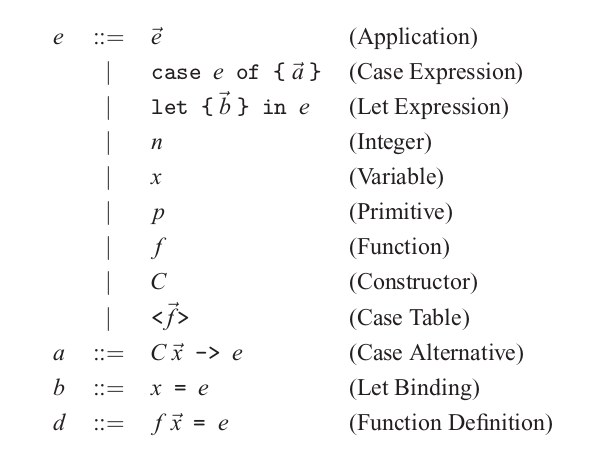
\includegraphics[scale=0.4]{core_syntax}
\label{fig:core_syntax}
\caption{Синтаксис ядра языка F-lite.}
\end{figure}

\section{Компиляция}
Эта секция определяет набор уточнений, которые приводит программу, написанну на ленивом языке программирования F-lite, к форме, известной как \textit{шаблонный код} (template code), которую Редуцерон может исполнять.

\subsection{Исходный язык}
F-lite является ядровым ленивым функциональным языком, близкий к подмножествам как Haskell так и Clean. Синтакс F-lite представлен на рис.~\ref{fig:core_syntax}.

\textbf{Частные выражения (case expressions).} Частные выражения представлены в упрощенной форме, которая может быть получена с помощью компилятора шаблонного поиска (pattern match compiler) такого как тот, который определен в Peyton Jones (1987). Шаблоны в частных выражениях являются конструкторами, примененными к нулю или более переменным. Каждое частное выражение содержит альтернативу для каждого конструктора расматриваемого в выражении типа.

\textbf{Примитивы.} Мета-переменная \textit{p} обозначает символ примитивной функции. Все применения примитивных функций полностью насыщены (т.е. они не могут частично применяться, можно подать только столько переменных, сколько арность примитивной функции). Редуцерон реализует только малый набор примитивных операций, не полный набор традиционного процессора, как пример, отсутствуют операции с числами с плавающей запятой. В примитивы, используемые в данной статье, включаются (+), (-) и (<=).

\textbf{Main.} Каждая программа содержит определение главной функции \textit{main = e}, где e является выражением, которое вычисляется в целочисленное n; результат выполнения программы - значение n.

\textbf{Таблицы частных случаев (Case tables).} Отметьте необочную конструкцию для таблиц частных случаев $<\overrightarrow{f}>$. Таблицы частных случаев не пишутся в исходных программах, а появляются во время компиляции - смотри Главу 2.4.

\textbf{Примеры.} Ниже представлены два примера для определения функции. Первая соединяет два списка и вторая высчитывает треугольные числа.

\begin{verbatim}
append xs ys = case xs of
  { Nil -> ys ; Cons x xs -> Cons x (append xs ys) }
  
tri n = case (<=) n 1 of
  { False -> (+) (tri ((-) n 1)) n ; True -> 1 }
\end{verbatim}

\subsection{Терминология}
\textbf{Длина применения (Application length).} \textit{Длина} применения $e_1 \ldots e_n$ есть $n$. Для примера, длина применения \textit{append xs ys} - 3.

\textbf{Смешанные выражения (Compound expression) и атомарные выражения (atomic expressions).} Применения, частные выражения и выражения объявления (let expressions) являются смешанными. Все другие выражения являются атомарными.

\textbf{Плоские выражния (Flat expression).} Плоское выражение - это атомарное выражение или применение $e_1 \ldots e_n$, в котором каждое $e_i$ для $i \in [1 \ldots n]$ является атомарным выражением. Для примера, \textit{append xs ys} является плоским выражением, но \textit{tri ((-) n 1)} не является.

\textbf{Граф выражения (Expression graph).} Выражение объявления:
$$
let \; \{ x_1 = e_1 ; \ldots ; x_n = e_n \} \; in \; e
$$
является графом выражения тогда и только тогда, когда $e$ является плоским выражением и каждое $e_i$ для $i \in [1 \ldots n]$ является плоским выражением. Графы выражением являются ограниченной А-нормальными формами (Flanagan et al., 1993). 

\textbf{Индекс конструктора и арность.} Каждый конструктор $C$ типа данных с $m$ конструкторами связан с уникальным индексом в диапазоне $1 \ldots m$. Более точно, индекс конструктора является его позицией в отсортированном в алфавитном порядке списке всех конструкторов данного типа. Для примера, стандартный тип данных для списка имеет два конструктора: \textit{Cons} имеет индекс 1 и \textit{Nil} имеет индекс 2. Конструктор с индексом $i$ обозначается как $C_i$, и арность конструктора $C$ обозначается как $\#C$.

\subsection{Примитивные применения}
В ленивом языке применение примитивной функции такой как (+), (-) или (<=) требует специальной обработки: целочисленные аргументы должны быть полностью вычислены перед тем как применение будет редуцировано. Один из простых подходов является трансформация бинарного примитивного применения с помощью правила:
\begin{equation} \label{eq:rule_primitive_applications}
p \; e_0 \; e_1 \rightarrow e_1 \; (e_0 \; p)
\end{equation}

вместе с правилом редукции во время исполнения:
\begin{equation} \label{eq:reduce_primitive_applications}
n \; e \rightarrow e \; n
\end{equation}

для полностью вычисленного целочисленного литерала $n$. Для иллюстрации данного подхода, рассмотрим выражение \textit{(+) (tri 1) (tri 2)}. Благодаря применению правила (\ref{eq:rule_primitive_applications}) во время компиляции, выражение трансформируется в \textit{tri 2 ((tri 1) (+))}. Во время исполнения, редукция проводится следующим образом:

\begin{align*}
& tri \; 2 \; ((tri \; 1) \; (+)) & \{ tri \; 2 \; \text{вычисляется в} \; 3 \} & \\
& = 3 \; ((tri \; 1) \; (+)) & \{ \text{Правило (2)} \} & \\
& = (tri \; 1) \; (+) \; 3 &  \{ tri \; 1 \; \text{вычисляется в} \; 1 \} & \\
& = 1 \; (+) \; 3 & \{ \text{Правило (2)} \} & \\
& = (+) \; 1 \; 3
\end{align*}

После трансформации с помощью правила (\ref{eq:rule_primitive_applications}), \textit{tri} выглядит как:
\begin{verbatim}
tri n = case 1 (n (<=)) of
  { False -> n (tri (1 (n (-))) (+)) ; True -> 1 }
\end{verbatim}

В Главе 5, мы представляем более эффективные техники для работы с примитивными применениями.

\subsection{Частные применения (Case expressions)}
Эта глава описывает как частные выражения компилируются. Сперва расмотрим кодирование по Скотту (Scott, 1968) недавно переоткрытое Jansen et al (2007). После этого дадим несколько уточнений для данного кодирования.

\textbf{Кодирование по Скотту/Янсену.} Первый шаг кодирования - генерация для каждого конструктора $C_i$ типа данных с $m$ конструкторами определения фукцнии:
\begin{equation} \label{eq:scott_encoding_1}
C_i \; x_i \ldots x_{\#C_i} \; k_1 \ldots k_m = k_i \; x_1 \ldots x_{\#C_i}
\end{equation}

Идея в том, что каждый конструктор данных $C_i$ закодирован как функция, которая берет как аргументы $\#C_i$ аргументов конструктора и $m$ продолжений (continuations). Функция, кодирующая конструктор $C_i$, передает аргумента конструктора i-тому продолжениюю Для примера, конструкторы списка трансформируются в следующие функции:

\begin{verbatim}
Cons x xs c n = c x xs
Nil       c n = n
\end{verbatim}

Теперь частное выражение следующей формы:
\begin{equation} \label{eq:scott_encoding_2}
case \; e \; of \; \{ \; C_1 \; \overrightarrow{x_1} \; \rightarrow e_i ; \ldots ; \; C_m \; \overrightarrow{x_m} \rightarrow e_m \; \}
\end{equation}

трансформируется в:
$$
e (alt_1 \;  \overrightarrow{v_1} \; \overrightarrow{x_1} ) \ldots (alt_m \;  \overrightarrow{v_m} \; \overrightarrow{x_m} )
$$
, где $\overrightarrow{v_i}$ - свободные переменные, появляющиеся в i-той частной альтернативе и каждый $alt_i$ для $i \in [1 \ldots m]$ имеет определение:

$$
	alt_i \; \overrightarrow{v_i} \; \overrightarrow{x_i} = e_i
$$

Для примера, функция \textit{append} трансформируется в:
\begin{verbatim}
append xs ys = xs (consCase ys) (nilCase ys)
consCase ys x xs = Cons x (append xs ys)
nilCase  ys      = ys
\end{verbatim}

Заметьте, что применение \textit{nilCase} можно редуцировать во время компиляции. Это следствии того, что конструктор \textit{Nil} имеет арность 0.

\textbf{Пример побольше.} Теперь посмотрим на немного больший пример: Вычисление базовых арифметических выражения.
\begin{verbatim}
eval x y e = case e of {
  Add n m -> (+) (eval x y n) (eval x y m);
  Neg n   -> (-) 0 (eval x y n);
  Sub n m -> (-) (eval x y n) (eval x y m);
  X       -> x;
  Y       -> Y;
}
\end{verbatim}

После пробразования и подстановки (in-lining) нулевых случаев, мы имеем:
\begin{verbatim}
eval x y e = e (add x y) (neg x y) (sub x y) x y
add  x y n m = (+) (eval x y n) (eval x y m)
neg  x y n   = (-) 0 (eval x y n)
sub  x y n m = (-) (eval x y n) (eval x y m)
\end{verbatim}

Посмотрите на огромное тело \textit{eval}: оно содержит три вложенных применений функций и несколько повторяющихся ссылок на $x$ и $y$. В типичной реализации фунационального языка программирования большие тела функций более дороги для создания, чем маленькие.

\subsection{Уточнение 1.} 
\end{document}